\Def Дерево отрезков (англ. Segment tree) — это структура данных, которая позволяет за асимптотику $O(log(n))$ реализовать любые операции, определяемые на множестве, на котором данная операция ассоциативна, коммутативна и имеет нейтральный элемент относительно этой операции.

В частности, задачи RSQ/RMQ, как правило, решается с использованием этой структуры данных.

\begin{center}
 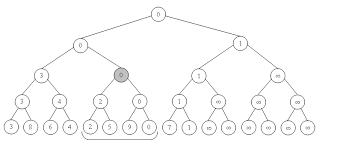
\includegraphics[width = 10cm]{pix/stree.png}    
\end{center}

\subsubsection{Построение}
Опишем нерекурсивное построение дерева на массиве длины N.

\begin{enumerate}
    \item Будем считать, что $log_2\,N \in \N$, иначе дозаполним до степени двойки нейтральными элементами.
    \item Заведем массив длины $2N - 1$, последние $N$ элементов будут элементами исходного массива.
    \item Первые $N - 1$ элементов заполним следующим образом:\\
    $t[i]\,=\,F(t[2i + 1],\,t[2i + 2])$ (заполнение от элемента с номером N - 2 и до 0 в цикле).
\end{enumerate}

\subsection*{Изменение в точке}

Пусть необходимо обновить элемент с индексом i.
\begin{enumerate}
    \item Найдем в дереве лист, отвечающий за i-й элемент. Это $(N - 1 + i)$-й.
    \item Индекс родителя $\lfloor \frac{N - 2 + i}{2} \rfloor$ (Если корень в вершине с номером 0)
    \item Обновляем значение в родителе через результаты на деревьях.
    \item Повтори, пока не обновил корень.
\end{enumerate}

\subsubsection*{Ответ на запрос}
Пусть мы находимся в узле, отвечающего за подотрезок $[l,\,r]$, а изначальный запрос был $[L,\,R]$.

\begin{enumerate}
    \item Если $[l,\,r] \cap [L,\,R] = \varnothing$, то вернем нейтральный элемент.
    \item Если $[l,\,r] \subseteq [L,\,R]$, то вернем значение в узле.
    \item Иначе вернем результат операции с детей.
\end{enumerate}

\textbf{Асимптотика} Заметим, что на каждом уровне раскрываться вниз могут не более двух узлов, так как только крайние могут порождать дочерние запросы. Следовательно, время работы $O(log\,N)$.

\pagebreak